\providecommand{\isolatedBuild}[1]{#1}% fallback definition lets this file build normally
\isolatedBuild
{
\documentclass[11pt,letterpaper]{book}
\usepackage{import}

% This file must be found via the TEXINPUTS environment variable.
%\documentclass[11pt,letterpaper]{book}

% aleeper: I think these are needed for Paul's macros?
\usepackage{epsfig}
\usepackage{epstopdf}

%\makeatletter
%\typeout{The import path is \import@path}
%\makeatother

\usepackage{import}

\subimport{./}{packagesMitiguy.sty}
\subimport{./}{macrosMitiguy.tex}
\subimport{./}{PageStylesMitiguy.tex}
\subimport{./}{macrosLeeper.tex}


\pagestyle{plain}
\pagenumbering{arabic}

\begin{document}
\HandoutHeader{Robots Are Awesome}
%
%\vspace{-0.5pc}
\normalsize
\textColorBold{darkerBlue}{Statics of a Welding Robot}
\\[0.45pc]
}
%%%%%%%%%%%%%%%%%%%%%%%%%%%%%%%%%%%%%%%%%%%%%%%%%%%%%%%%%%%
%
Consider the 3-\textit{degree-of-freedom} (3-DOF) welding robot
consisting of a grounded link, \basis{N}, and rigid links \basis{A}, \basis{B}, and \basis{C}.
Revolute torque motors connect the links at points $A_o$, $B_o$, and $C_o$.
\\[0.45pc]
\begin{minipage}[b]{0.47\linewidth}
%
\begin{itemize}
\item \boldUnderlineDarkRed{Draw} a right-handed, unitary, orthogonal basis \uvecBasisxyz{a} \textit{initially aligned} with \uvecBasisxyz{n}.
Basis \uvecBasisxyz{a} is then
subjected to a $+\uvecy{a}$ rotation of $\theta_A$ (don't draw that; it simply changes the ``plane" in which links \basis{B} and \basis{C} operate.)

\item \boldUnderlineDarkRed{Draw} a right-handed, unitary,
orthogonal basis \uvecBasisxyz{b} fixed on body \basis{B}
\textit{initially aligned} with \uvecBasisxyz{a} and then subjected
to a $+\uvecz{b}$ rotation of $\theta_B$.

\item \boldUnderlineDarkRed{Draw} a right-handed, unitary,
orthogonal basis \uvecBasisxyz{b} fixed on body \basis{C}
\textit{initially aligned} with \uvecBasisxyz{b} and then subjected
to a $-\uvecz{c}$ rotation of $\theta_C$.
\end{itemize}
%
\vspace{0.5pc}
Link A has mass $m^A = 60$ kg.
\\[0.0pc]
Link B has mass $m^B = 40$ kg and length $L_B = 1.0$ m.
\\[0.0pc]
Link C has mass $m^C = 30$ kg and length $L_C = 0.8$ m.
\\[0.0pc]
A force with magnitude $F_T = 500$ N acts perpendicular to link \basis{C}, as shown.
\end{minipage}
\hfill
\begin{minipage}[b]{0.48\linewidth}
\flushright
\vspace*{-0pc}
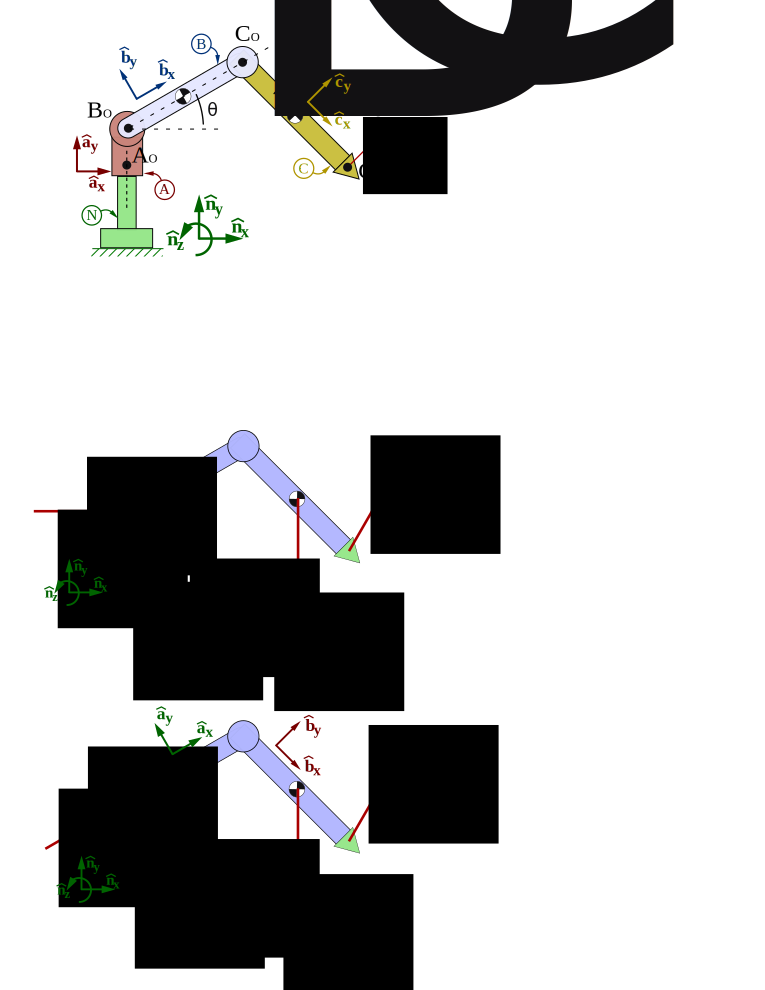
\includegraphics[width=0.99\linewidth]{robot.png}
\end{minipage}
\\[1.0pc]
Complete the following rotation tables. (You may use the space below to
\boldUnderlineDarkRed{re-draw} the bases to help you).
\\[0.45pc]
\begin{minipage}{0.33\linewidth}
{
\large
\rotationTableEmpty{a}{n}{\hspace{1.0cm}}
}
\end{minipage}
\begin{minipage}{0.33\linewidth}
{
\large
\rotationTableEmpty{a}{b}{\hspace{1.0cm}}
}
\end{minipage}
\begin{minipage}{0.33\linewidth}
{
\large
\rotationTableEmpty{b}{c}{\hspace{1.0cm}}
}
\end{minipage}
%
%\\[2.0pc]
%\begin{minipage}{0.33\linewidth}
%{
%\rotationTable{a}{c}
%{~\cos(\theta_B - \theta_C)}{~-\sin(\theta_B - \theta_C)}{0}
%{~\sin(\theta_B - \theta_C)}{~~~\cos(\theta_B - \theta_C)}{0}
%{0}{0}{1}
%}
%\end{minipage}
\\[8.0pc]
\vfill
\begin{enumerate}
\item \textbf{Explain} how to obtain the rotation table \dircos{n}{c} using only the tables above. (You don't need to carry it out.)
\\[2.0pc]
\item Assume the torque motors act to hold the robot fixed in the configuration shown (including the load $F_T$). Assume a 2-D problem (so we can ignore out-of-plane forces/torques).
\boldUnderlineDarkRed{Draw} a FBD of each of the following systems. \boldUnderlineDarkRed{State} your assumptions. In each case, how many unknown force/torque measures do you introduce?
\begin{enumerate}
\item \basis{S} consists of link \basis{C}.
\item \basis{S} consists of links \basis{B} and \basis{C}.
\item (\textbf{Optional, 3D}) \basis{S} consists of links \basis{A}, \basis{B}, and \basis{C}.
\end{enumerate}
%
%\clearpage
%\item You are asked to make sure the shoulder joint (located at point $A_o$) is sufficiently strong to support the rest of the arm. \boldUnderlineDarkRed{Draw} a FBD of the system consisting of $A$ and $B$. How many unknowns does this require you to introduce? Using $\force{S} = \bvec{0}$, \boldUnderlineDarkRed{calculate} the magnitude of the reaction force at the shoulder.
%\\[0.45pc]
%\item Consider the same system as before ($A$ + $B$).
%Now what you care about is the \textit{axial} force in link $A$ right by the shoulder joint.
%\boldUnderlineDarkRed{Draw} a FBD of the system consisting of $A$ and $B$.
%Using $\force{S} = \bvec{0}$, \boldUnderlineDarkRed{calculate} the axial force at the shoulder.
\end{enumerate}
%
%
\isolatedBuild {
\vfill
\end{document} }
